\documentclass{article} % lub inna klasa dokumentu, np. report lub book
\usepackage[utf8]{inputenc} % ustawienie kodowania na UTF-8
\usepackage{amsmath, amssymb, amsthm} % biblioteki do działań matematycznych
\usepackage[T1]{fontenc}    % wybór odpowiedniego kodowania czcionek
\usepackage{polski}         % dodanie wsparcia dla polskich znaków
\usepackage{babel}          % automatyczne dostosowanie języka
\usepackage{pgfplots}       % Pakiet do tworzenia wykresów
\usepackage{verbatim}
\usepackage{esvect}
\pgfplotsset{compat=1.18}

\title{Sprawozdanie}

\author{Tomasz Lisowski 197749\and Filip Świniarski 197725\and Nikodem Miłuch 197922}


\begin{document}
\maketitle


\section{Zadanie E5.1}
\subsection{Opis}

Zadanie polega na narysowaniu wykresu zależności $F = f(I)$ dla stałej wartości indukcji pola magnetycznego. Jako pomiar przyjęto wskazanie wagi w czasie, gdy obwód elektryczny był zamknięty. Ponieważ waga była zrównoważona przed zamknięciem obwodu, wynik wagi jest proporcjonalny do natężenia prądu płynącego w przewodzie.

\subsection{Wzory}
Wartość siły elektrodynamicznej dana jest wzorem:
{\large
\begin{equation}
    F = IlB\sin{a} 
\end{equation}}
ponieważ $\alpha = 90$° wartość sinusa jest równa 1. Z prawa powszechnego ciążenia otrzymujemy:
{\large
\begin{equation}
    F = mg 
\end{equation}}
\subsection{Wykres}
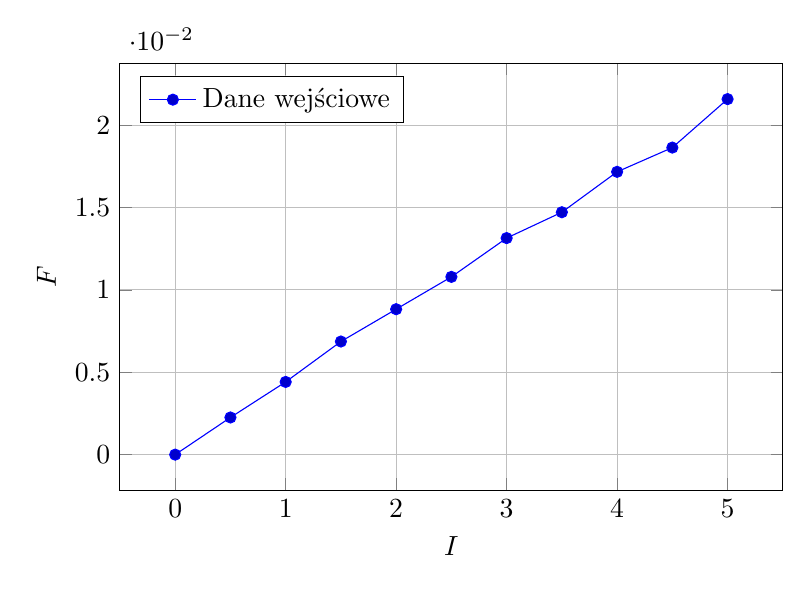
\begin{tikzpicture}
    \begin{axis}[
        xlabel={$I$},
        ylabel={$F$},
        grid=major,
        width=10cm,
        height=7cm,
        legend pos=north west,
    ]
    % Dane
    \addplot coordinates {
        (0, 0.0)
        (0.5, 0.0022563)
        (1, 0.0044145)
        (1.5, 0.006867)
        (2, 0.008829)
        (2.5, 0.010791)
        (3, 0.0131454)
        (3.5, 0.014715)
        (4, 0.0171675)
        (4.5, 0.018639)
        (5, 0.021582)
    };
    \legend{Dane wejściowe}
    \end{axis}
\end{tikzpicture}
\section{Zadanie E5.2}
\subsection{Opis}

Zadanie polega na wyznaczeniu wartości indukji magnetycznej pola w szczelinie magnesu, wykorzystując przy tym wykres z poprzedniego punktu.

\subsection{Wyznaczenie współczynnika kierunkowego}

Korzystając z wykresu wyznaczamy współczynnik kierunkowy jako:
{\large
\begin{equation}
    a= \frac{\Delta x}{\Delta y} = \frac{0.021582}{5} = 0.0043164
\end{equation}
}
\subsection{Błąd pomiarowy}
Przyjmujem, że $\Delta I = 0.01A$ a $\Delta m = 0.01g$. Podstawiając te dane do wzoru na niepewność wielkości złożonej otrzymujemy:
{\large
\begin{equation}
    a = 0.0043164\pm 0.0000089
\end{equation}
}
\subsection{Wyznaczenie indukcji pola}
Ponieważ:
{\large
\begin{equation}
    B = \frac{a}{l}
\end{equation}
}
oraz:
{\large
\begin{equation}
    S_b = \frac{S_a}{l}
\end{equation}
}
Podstawiając dane z wzoru (3) do wzoru (5) i (6) otrzymujemy ($l = 0.1m$):

{\large
\begin{equation}
    a = 0.043164\pm0.000089
\end{equation}
}
\section{Zadanie E5.3}

\subsection{Opis}

Poprzez wykonwyanie pomiarów w obwodzie, w kótrym płynął prąd o stałym napięciu, ale zwiększającej się mocy otrzymujemy zależność wartości indukcji pola magnetycznego $B$ od nateżenie prądu płynącego przez zwojnicę.
\subsection{Wzory}

Do obliczenia wartości indukcji pola magnetycznego wykorzystujemy zależność:
{\large
\begin{equation}
    B = \frac{F}{Il}
\end{equation}
}

\subsection{Wykres}

Pomiar wykonano przy stałym natężeniu $I = 2$A. 
Dane pomiarowe przedstawia wykres poniżej:

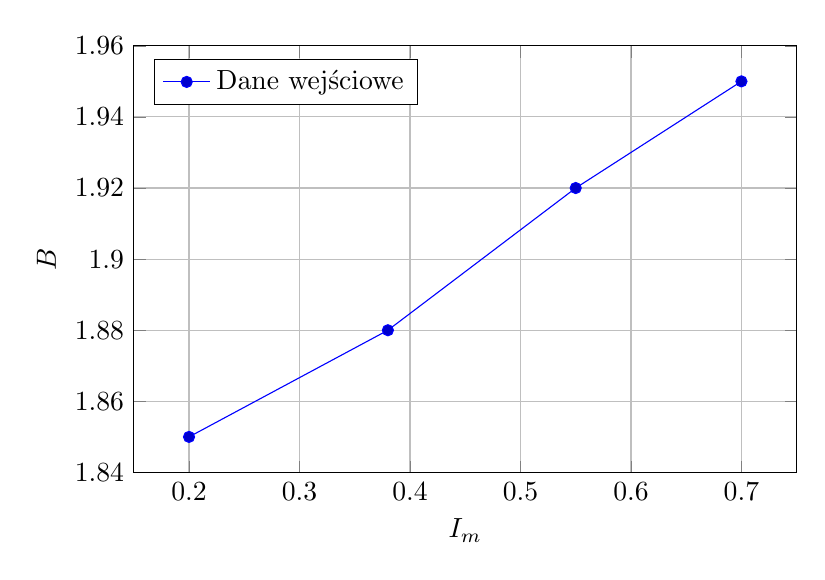
\begin{tikzpicture}
    \begin{axis}[
        xlabel={$I_m$},
        ylabel={$B$},
        grid=major,
        width=10cm,
        height=7cm,
        legend pos=north west,
    ]
    % Dane
    \addplot coordinates {
        (0.2, 1.85)
        (0.38, 1.88)
        (0.55, 1.92)
        (0.7, 1.95)
    };
    \legend{Dane wejściowe}
    \end{axis}
\end{tikzpicture}
\section{Wnioski}

Dane wahają się znaczenie z uwagi na niedokładność sprzętu laboratoryjnego.

\end{document}

